\section{基于群智协同的众包测试}

\subsection{众包测试流程}
\begin{itemize}
    \item 申请上传:用广将自己的应用程序上传到众测平台,并指定相应的测试任务和酬劳信息。
    \item 任务选择和环境设置:众测人员自由选择他们想要完成的任务。选择后测试人员从平台上下载应用程序进行测试。
    \item 提交报告:众测人员根据选择的待测应用,对测试到的缺陷提交缺陷报告。
    \item 生成最终测试报告:平台收集补充信息,生成最终的缺陷报告,包括:一般信息、设备信息、操作路径等。
    \item 报告验证:客户将验证所有最终的缺陷报告,并决定如何酬劳每个提交报告的众包测试人员。
\end{itemize}

\begin{figure}[H]
    \vspace{-0.5em}
	\centering
	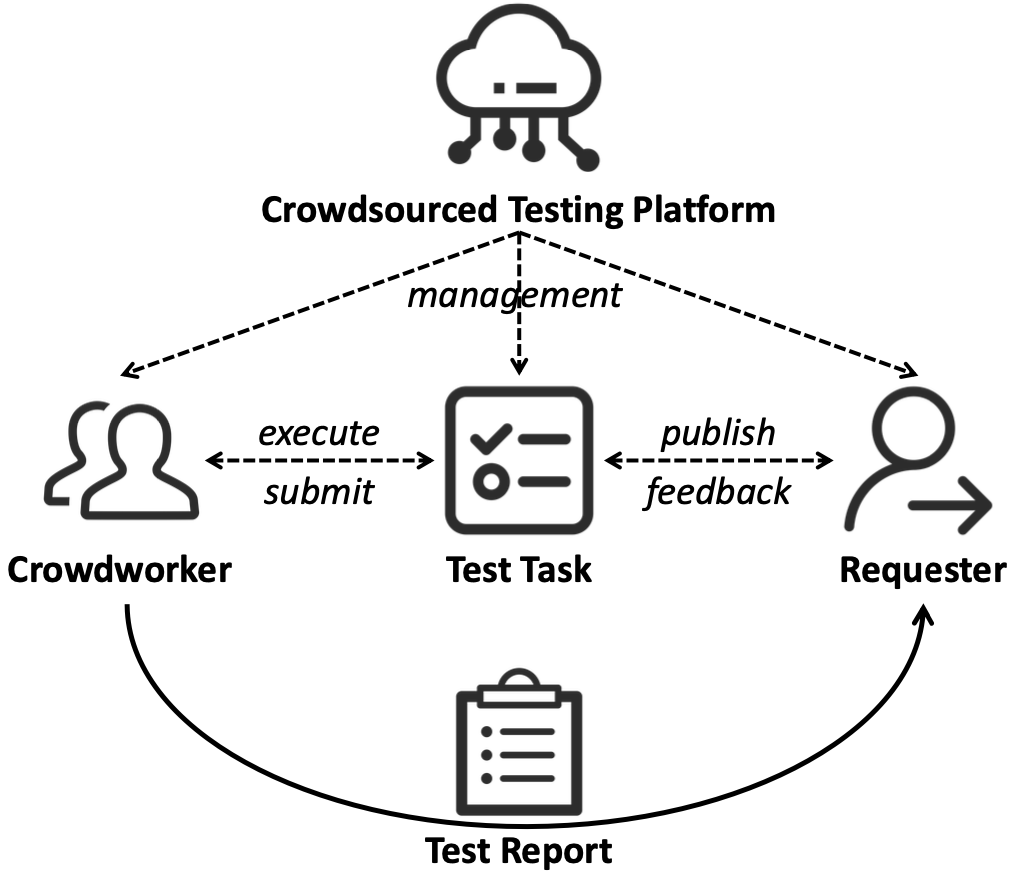
\includegraphics[width=0.4\textwidth]{images/众包测试流程.png}
    \vspace{-1em}
\end{figure}

\subsection{众包测试的特点}

众包测试的优势
\vspace{-0.5em}
\begin{multicols}{2}
    \begin{itemize}
        \item 更充分的测试时间
        \item 更广泛的测试方法
        \item 更多样的测试环境
        \item 更全面的测试覆盖
    \end{itemize}
\end{multicols}
\vspace{-1em}

众包测试面临的挑战
\vspace{-0.5em}
\begin{multicols}{2}
    \begin{itemize}
        \item 任务分配
        \item 任务奖励
        \item 众测过程引导
        \item 测试报告质量控制
    \end{itemize}
\end{multicols}
\vspace{-1em}

\subsection{对于众包测试存在的问题的解决}
协作式众包测试
\begin{itemize}
    \item 完成测试任务过程中进行信息共享与任务分配,用户在本系统中既承担测试任务也承担审核任务,充分利用用户协作,完成目标任务。
    \item 信息共享:用户在提交报告时进行实时相似报告推荐,避免重复报告提交。
    \item 任务分配:审核页面推荐待审核的报告列表,测试页面推荐待测页面。
    \item 协作方式:点赞点踩操作:利用用户的交叉审核,验证报告有效性。
    \item 一键Fork:Fork他人结果后进行修改,利用多人协作提升报告质量。
\end{itemize}

众测报告质量优化方法:文本和图像处理方法
\begin{itemize}
    \item 众测报告聚合
    \begin{itemize}
        \item Aggregator:对所有的测试报告做聚类,将相同的或相似的测试报告聚为同类。
        \item Summarizer:对每一类测试报告做整合,将其中的相关信息以可视化的方式最大化的呈现给开发者。
    \end{itemize}
    \item 众测报告排序
    \item 深度众测报告排序
    \item 众测报告半监督聚类
    \item 众测报告一致性检测
\end{itemize}


